\documentclass[crop=false]{standalone}
% --- ПРЕАМБУЛА ДЛЯ ПОДДЕРЖКИ РУССКОГО ЯЗЫКА И МАТЕМАТИКИ ---
\usepackage[T2A]{fontenc}
\usepackage[utf8]{inputenc}
\usepackage[russian]{babel}
\usepackage{amsmath}
\usepackage{geometry}
\usepackage{amssymb}
\usepackage{graphicx}
\usepackage{float}
\usepackage{import}
\geometry{a4paper, top=2cm, bottom=2cm, left=2cm, right=2cm}
\newcommand{\sidecomment}[1]{\marginpar{\raggedright\scriptsize\itshape #1}}
\newcommand{\iu}{\mathrm{i}}

\newcommand{\Def}{%
    \text{Def}%
    \hspace{-0.85em}% Сдвиг назад ровно на середину (подберите под шрифт)
    \raisebox{0.1ex}{/}% Черта
    \hspace{1em}% Возврат к концу слова + небольшой отступ
}

\renewcommand{\Re}{\operatorname{Re}}
\renewcommand{\Im}{\operatorname{Im}}

\ifstandalone
    \newcommand{\lecturebreak}{} % В отдельном файле лекции разрыв не нужен
\else
    \newcommand{\lecturebreak}{\clearpage} % В полной книге - начинаем с новой страницы
\fi

\newcounter{lecturenumber} % Создаем счетчик для нумерации лекций
\newcommand{\lecture}[2]{
    \lecturebreak
    \refstepcounter{lecturenumber} % Увеличиваем счетчик на 1
    \par\vspace{2em}\noindent % Отступ сверху и убираем абзацный отступ
    {\Large\bfseries % Делаем заголовок крупным и жирным
    Лекция \thelecturenumber: #1 % Выводим "Лекция N: Тема"
    \hfill % Растягиваем пробел, чтобы дата была справа
    \large\textit{#2}} % Выводим дату курсивом
    \par\vspace{1em} % Небольшой отступ снизу
    \addcontentsline{toc}{section}{Лекция \thelecturenumber: #1} % Добавляем в оглавление
    \par
}

\newcommand{\TwoCols}[2]{%
  \par\noindent % Начать с новой строки без отступа
  \begin{minipage}[t]{0.48\textwidth}
    #1
  \end{minipage}% <-- Важный '%' для удаления пробела
  \hfill % Растягивающийся пробел между колонками
  \begin{minipage}[t]{0.48\textwidth}
    #2
  \end{minipage}% <-- Важный '%' для удаления пробела
  \par%
}

\pagestyle{plain} % Включаем нумерацию страниц\
\begin{document}
\lecture{Ограничения накладываемые связями на скорости и ускорения точек механической системы}{03.03}
\section{Ограничения}
$N, \bar r_k, k = 1, \dots , N$

$(1) f_p(r_k ,t) =0 \quad p = 1, \dots P$ — геомеотрические связи

$(2) \sum_{k=1}^N a_{k s} \bar v_k + a_s = 0 \quad s = 1, \dots , S$ — дифференциальные связи(не интегрируемые)

Для геомеотрических:
\TwoCols{
\[\frac{d}{dt} f_p(\bar r_k, t)= 0\]
\[(3) \sum_{k=1}^N \frac{\partial f_p}{\partial \bar r_k} \bar v_k + \frac{\partial f_p}{\partial t} = 0\]
\[\sum_{k=1}^N \frac{\partial f_p}{\partial \bar r_k} \bar v_k = \begin{pmatrix}
    \frac{\partial f_p }{\partial x_k} \\
    \frac{\partial f_p }{\partial y_k} \\
    \frac{\partial f_p}{\partial y_k}
\end{pmatrix}
\cdot 
\begin{pmatrix}
    v_{x_k} \\
    v_{y_k} \\
    v_{z_k}
\end{pmatrix}
\]
}
{
    \[
    \begin{aligned}
    (4) \sum_{k=1}^N \frac{\partial f}{\partial \bar r_k} \bar w_k &+ \sum_{k=1}^N \sum_{l = 1}^{N} \frac{\partial^2 f}{\partial \bar r_l \partial \bar r_k} \bar v_k \bar v_l \\ &+ \sum_{k=1}^{N} \frac{\partial^2 f}{\partial \bar r_k \partial t} \bar v_k + \sum_{k=1}^{N} \frac{\partial^2 f}{\partial t \partial \bar r_k} \bar v_k + \frac{\partial^2 f_p }{\partial t^2}
    \end{aligned}
    \]
}

Для дифференциальной: 
\[(5) \sum_{k=1}^N \bar a_{k s} \bar w_k + \sum_{k=1}^N \sum_{l=1}^N \frac{\partial \bar a_{k s}}{\partial \bar r_l} \bar v_l \bar v_k + \sum_{k=1}^N \frac{\partial \bar a_{k s}}{\partial t} \bar v_k + \sum_{k=1}^N \frac{\partial a_{s}}{\partial \bar r_k} \bar v_k + \frac{\partial a_s}{\partial t} = 0\]

\Def Возможные положения — положения точки, удовлетворяющие связям

Будем обозначать возможные положения через $r_k^*$ — $(1)$

\Def Возможные скорости, возможные ускорение — аналогично

$v_k^*$ — $(2) (3)$

$w_k^*$ — $(4) (5)$

Возможное перемещение
$\Delta \bar r_k = \bar v_k^* d t$ — возможные перемещения

$d \bar r_k$ — действительные перемещения(движение, которое реализуется)
\begin{figure}[H] % сделать справа от текста
    \centering
    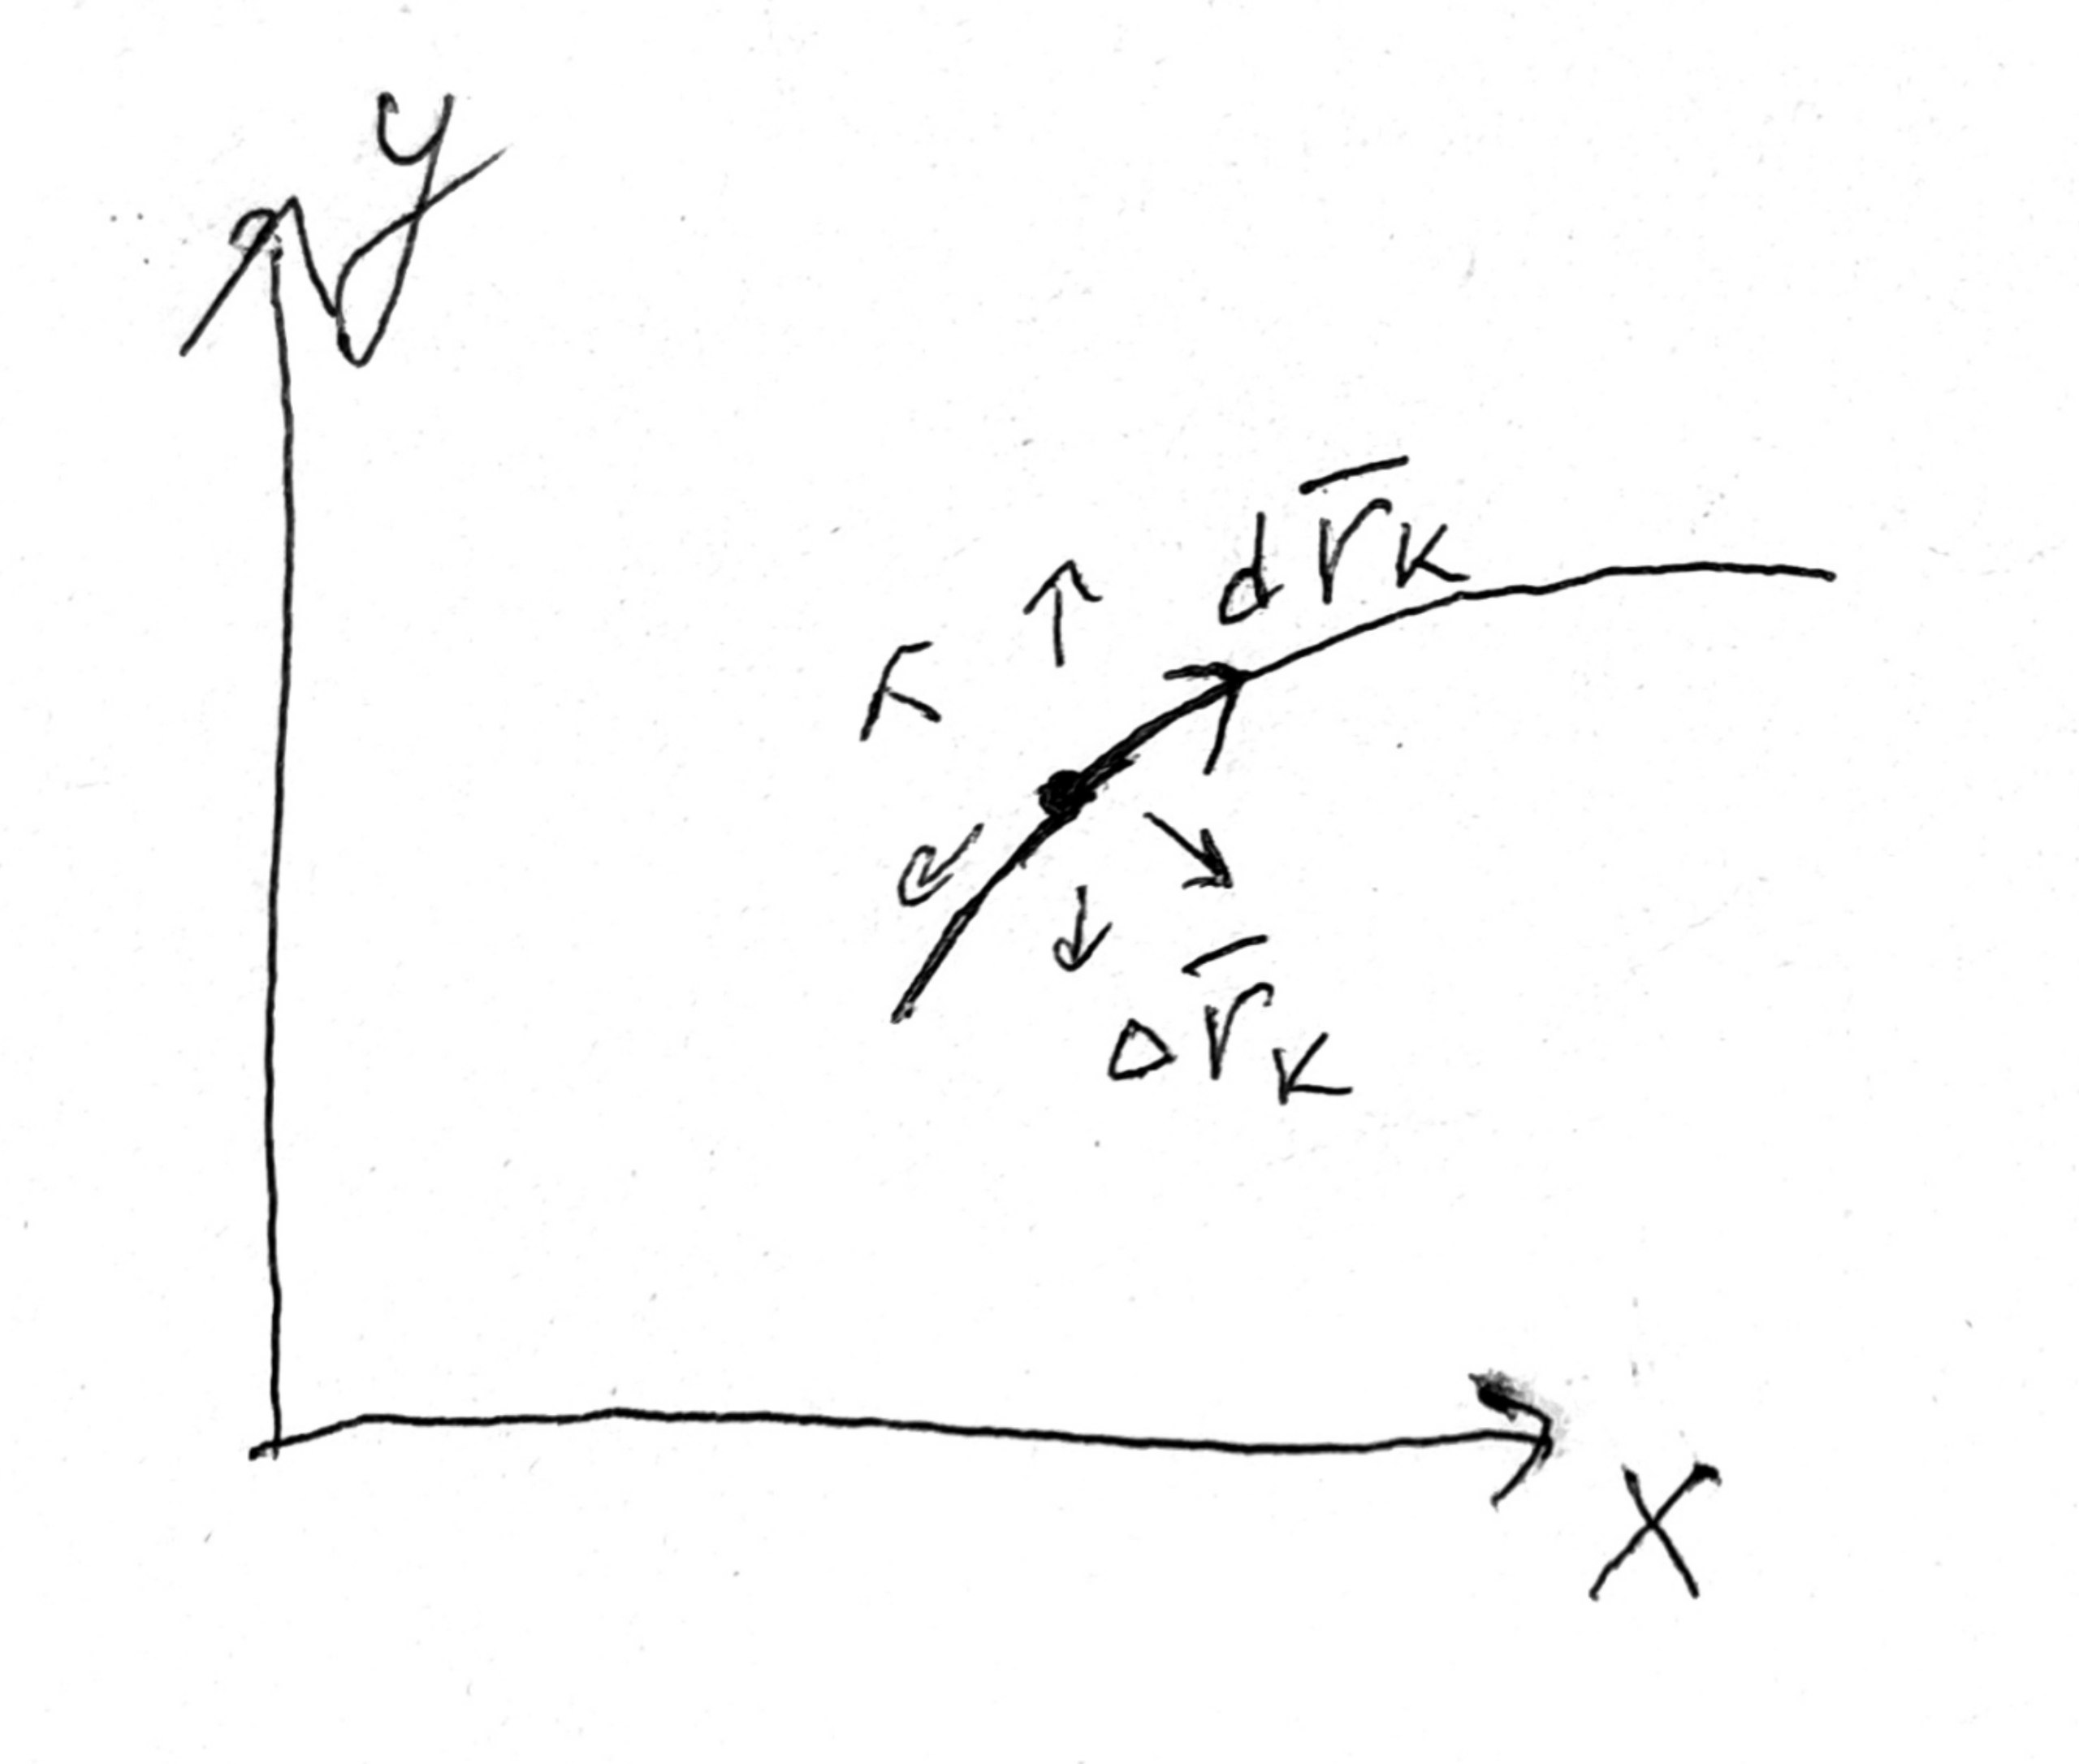
\includegraphics[width=0.5\textwidth]{possibleMovement.jpg}
    \caption{}
    \label{fig:myimage} % Sets a label for cross-referencing
\end{figure}

\Def Виртуальные перемещения $\delta \bar r_k$ — возможные перемещения, при зафиксированных связях(удовлетворяющие уравнению $(7)$)

\[(3) \sum_{k=1}^N \frac{\partial f_p}{\partial \bar r_k} \bar v_k + \frac{\partial f_p}{\partial t} = 0\]
\[\sum_{k=1}^N \frac{\partial f_p}{\partial \bar r_k} \bar v_k^* dt+ \frac{\partial f_p}{\partial t} dt = 0\]
\TwoCols{
    \[(6) \sum_{k=1}^N \frac{\partial f_p}{\partial \bar r_k} \bar \Delta \bar r_k^* + \frac{\partial f_p}{\partial t} dt = 0\]
\[\sum_{k=1}^N \frac{\partial f_p}{\partial \bar r_k} \bar \Delta \bar r_k^{**} + \frac{\partial f_p}{\partial t} dt = 0\]
}
{Вычитая уравнения друг из друга
    \[\sum_{k=1}^N \frac{\partial f_p}{\partial \bar r_k} (\Delta \bar r_k^* - \Delta r_k^{**}) + \frac{\partial f_p}{\partial t} dt = 0\]
    \[(7) \sum_{k=1}^N \frac{\partial f_p}{\partial \bar r_k} (\delta \bar r_k) + \frac{\partial f_p}{\partial t} dt = 0\]
}

для неголономных систем:

    \[(6) \begin{cases} \sum_{k=1}^N \frac{\partial f_p}{\partial \bar r_k} \bar \Delta \bar r_k^* + \frac{\partial f_p}{\partial t} dt = 0 \\
        \sum_{k = 1}^N \bar a_{k s} \Delta \bar r_k + a_s dt =0
    \end{cases}
\qquad (7) \begin{cases}
    \sum^N_{k = 1} \frac{\partial f_p}{\partial \bar r_k} \delta \bar r_k = 0 \\
    \sum_{k= 1}^N \bar a_{k s} \delta \bar r_k = 0
\end{cases}
\qquad \begin{matrix}
    \bar a_{k s} = \bar a_{k s} (\bar r_k, t) \\
    a_s = a_s(\bar r_k, t)
\end{matrix}
    \]
\keypoint Если связи стационарные, то возможные перемещния совпадают с виртуальными
\section{Обобщённые координаты}
Введём $q_1, \dots , q_m: \bar r_k = \bar r_k(q_1, \dots , q_m, t) \; (8)$ 
\Def эти $q_1, \dots, q_m$ называются обобщёнными коориднатами
$q_i(t)$ — закон движения
\[f_p(\bar r_k(q_1, \dots , q_m, t), t) = 0 \]
Пример:
\begin{figure}[H] % сделать справа от текста
    \centering
    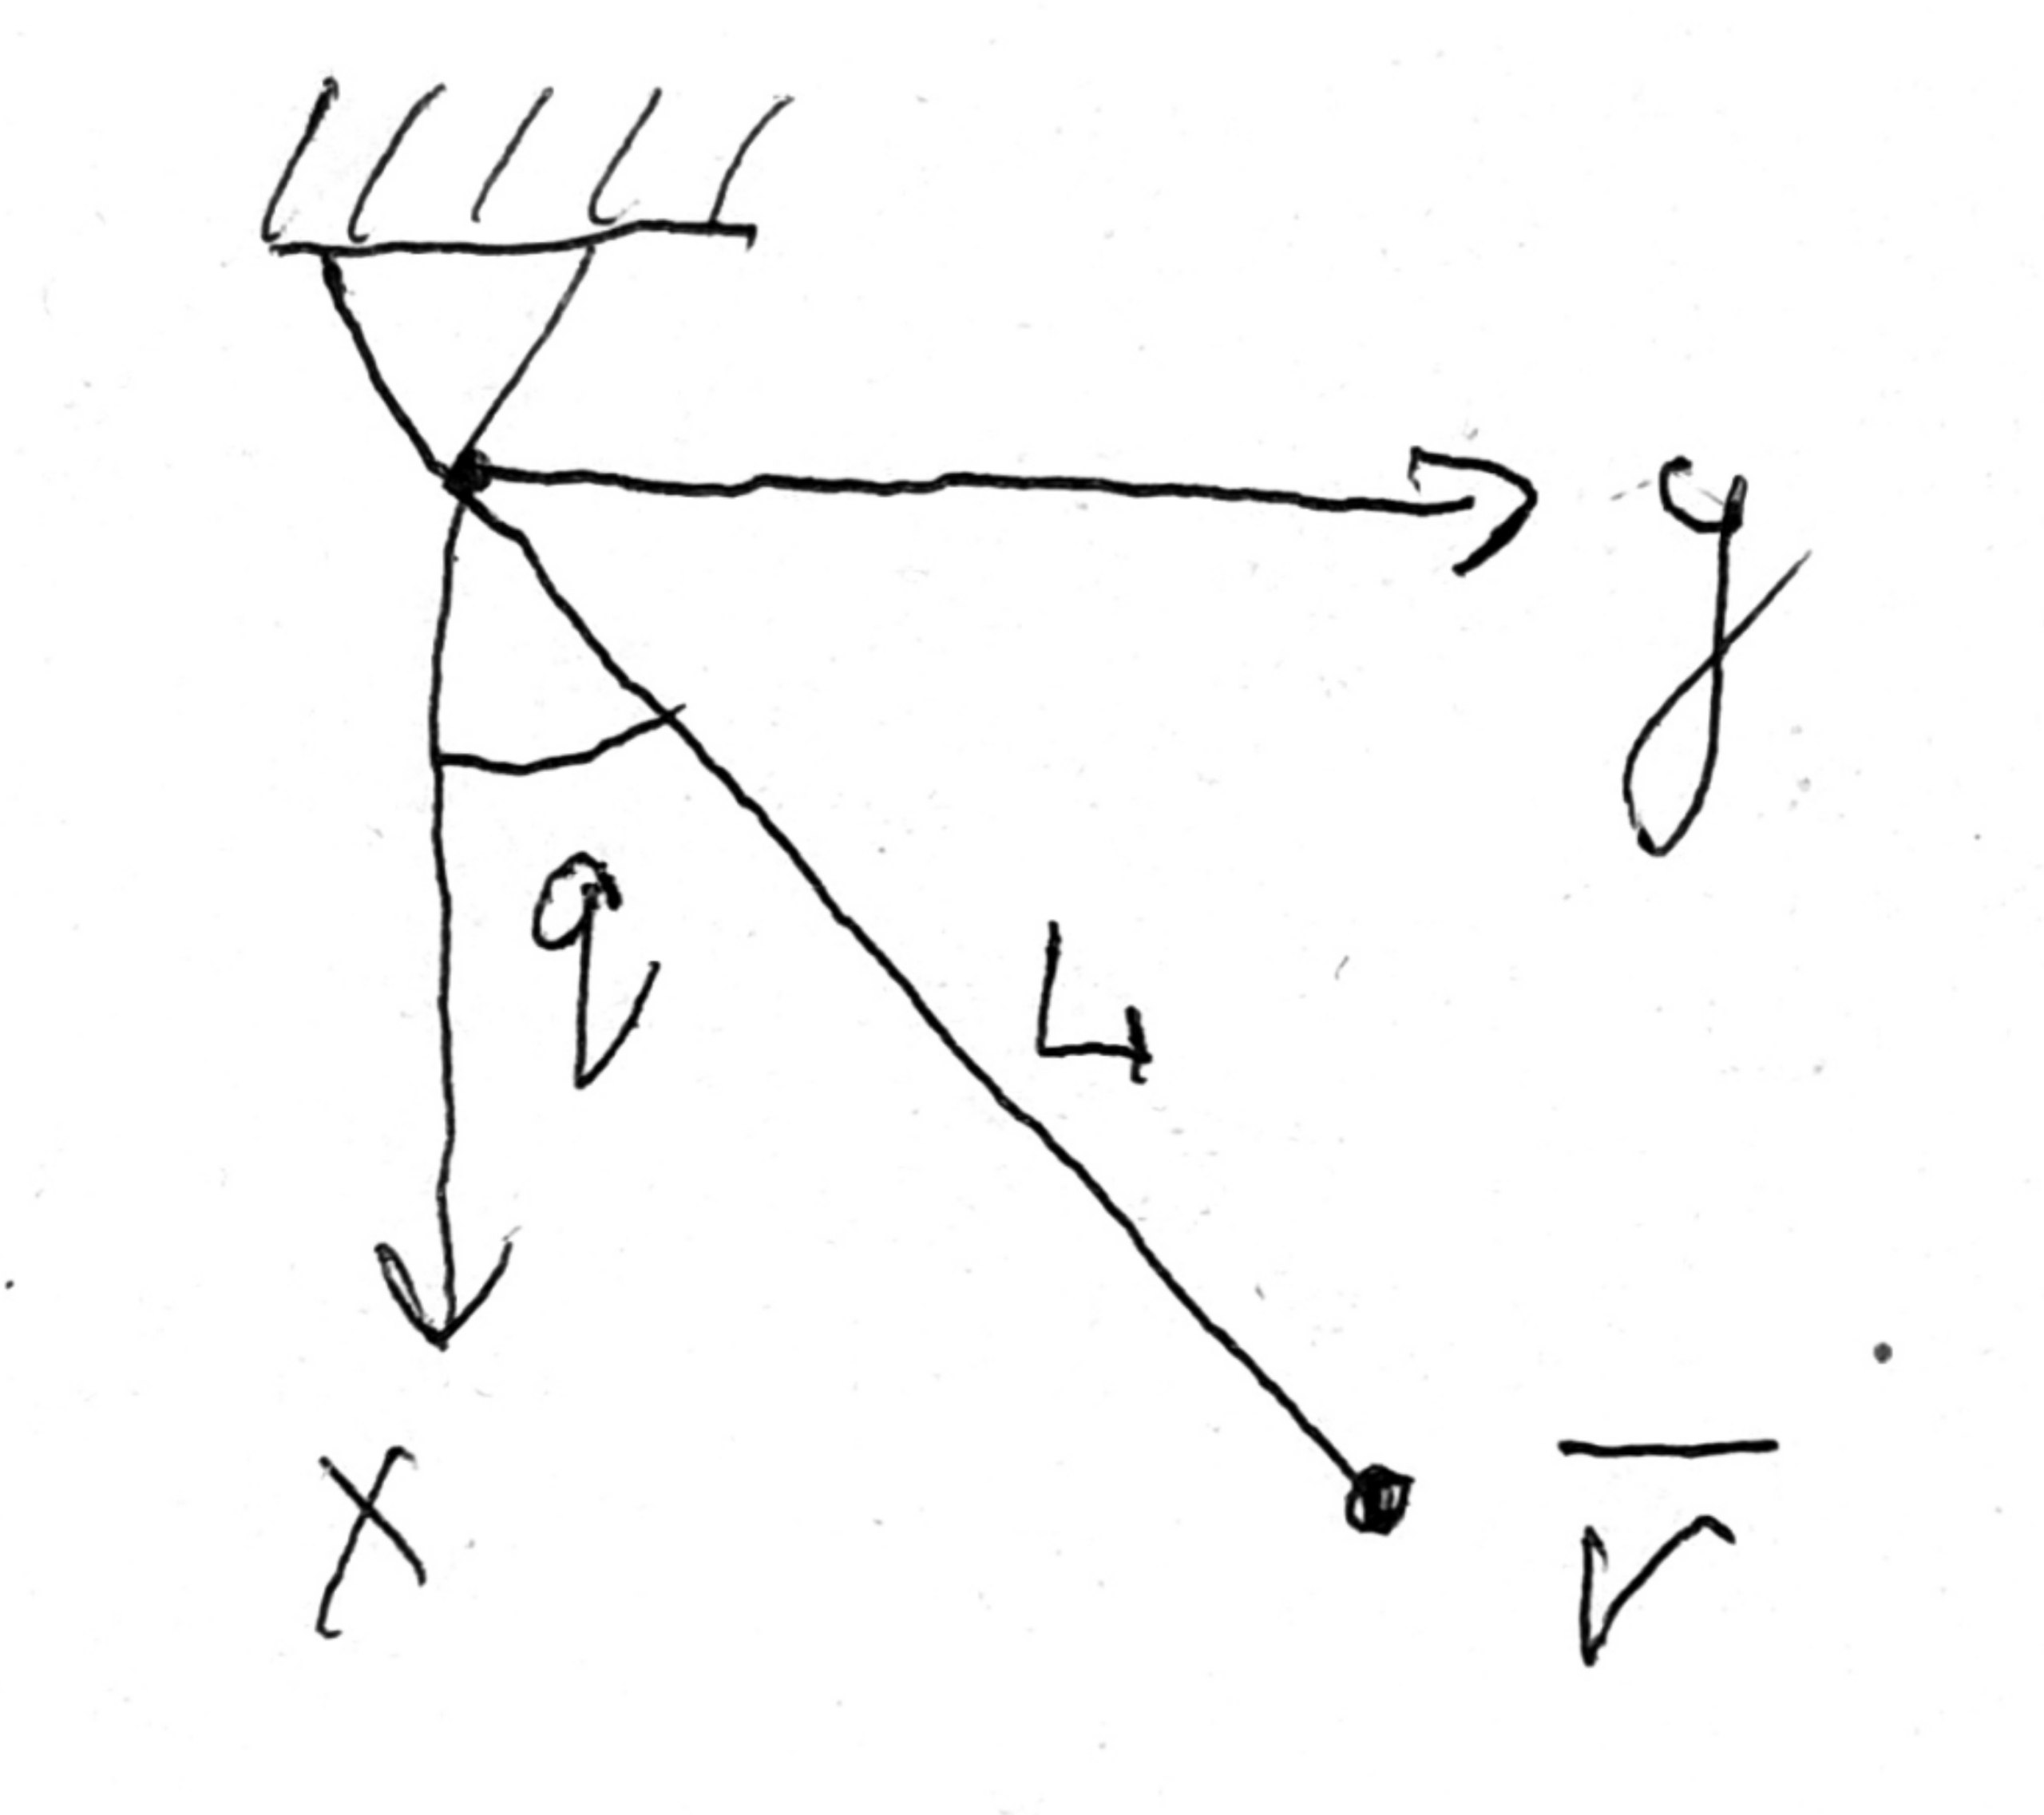
\includegraphics[width=0.5\textwidth]{unifiedCoordinates.jpg}
    \caption{}
    \label{fig:myimage} % Sets a label for cross-referencing
\end{figure}
\[N = 1 \qquad f(\bar r_k ,t ) = x^2 + y^2 - L^2 = 0 \qquad q: \begin{cases}
    x = L \cos q \\
    y = L \sin q 
\end{cases}
\]
\Def обобщённые скорости
\[\bar v_k = \dot{\bar r}_k = \sum_{k=1}^m \frac{\partial \bar r_k}{\partial q_i} \dot q_i + \frac{\partial \bar r_k}{\partial t}\]

\[\sum_{k=1}^N \bar a_{k s} \left(\sum_{i = 1}^N \frac{\partial \bar r_k }{\partial q_i} \dot q_i + \frac{\partial \bar r_k}{\partial t}\right) + a_s = 0\]
\[\sum_{i=1}^m \underbracket{\left(\sum_{k= 1}^N \bar a_{k s} \frac{\partial \bar r_k}{\partial q_i}\right)}_{b_{i s }} \dot q_i + \underbracket{\sum_{k=1}^N \bar a_{k s} \frac{\partial r_k}{\partial t} + a_s}_{b_s} = 0 \qquad (9) \sum_{i=1}^m b_{i s} \dot q_i + b_s = 0\]


Получилось что в голономной системе любая комбинация скоростей возможна(независимы), в неголономной должны удовлетворять $(9)$

\[\Delta \bar r_k = \Delta \bar r_k' - \Delta \bar r_k''  = \bar v_k^{*'} dt - \bar v_K^{*''} dt = \left(\sum_{i=1}^m \frac{\partial \bar r_k}{\partial q_i} \dot q_i' + \frac{\partial \bar r_k}{\partial t}\right)dt - \left( \sum_{i=1}^m \frac{\partial \bar r_k}{\partial q_i} \dot q_i'' + \frac{\partial \bar r_k}{\partial t}\right)dt = \sum_{i=1}^m \frac{\partial \bar r_k}{\partial q_i} (\dot q_i' - \dot q_i'') dt \] %fixme кривовато верхние индексы

\TwoCols{
\[\sum_{i= 1}^m b_{i s} \dot q_i ' dt + b_s dt = 0\]
\[\sum_{i =1 }^m  b_{i s} \dot q_i '' dt + b_s dt =0\]
}
{Вычитая получаем
\[\sum_{i=1}^{m} b_{i s} \underbracket{(\dot q_i ' - \dot q_i '' )}_{\delta q_i} dt = 0\]
}

\Def Число степеней свободы системы — количество её независимых виртуальных перемещений

обозначается $n = 3N - P - S$, $3$ — размерность пространства

В голономной системе $n =m$
\end{document}